\documentclass[12pt]{article}

% Packages 
\usepackage{amsmath}
\usepackage{datetime}
\usepackage{graphicx}
\usepackage{listings}
\usepackage{gensymb}

\graphicspath{{./images/}}

\newdate{date}{04}{04}{2022}
\title{
    Assignment 23

    \large{
        ME EN 6240 Advanced Mechatronics
    }  
}
    
\author{
        Ryan Dalby
}
\date{\displaydate{date}}

\setlength\parindent{0pt}

\begin{document}
\maketitle

\section*{Assignment 23}
See \verb|pidtest_plotting.m| for how these plots were generated.

\begin{enumerate}
    \item[a.] 

    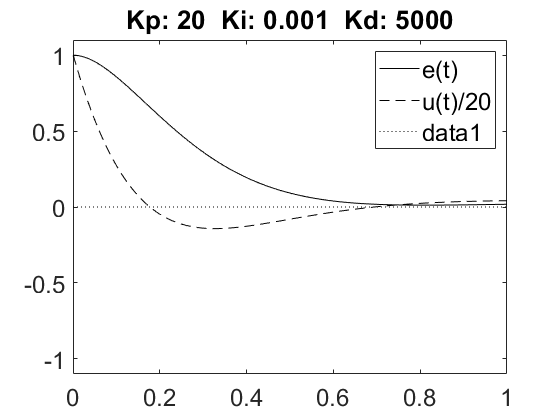
\includegraphics[width=4.8in]{23a.png}

    \item[b.] 
    The gains for the PID test with noise have to have derivative gains much lower than for the test without noise.
    Without noise it was possible to get a good response using a large $k_d = 5000$ value. 
    With the same gain values on the noisy system the response is unstable as can be seen below.

    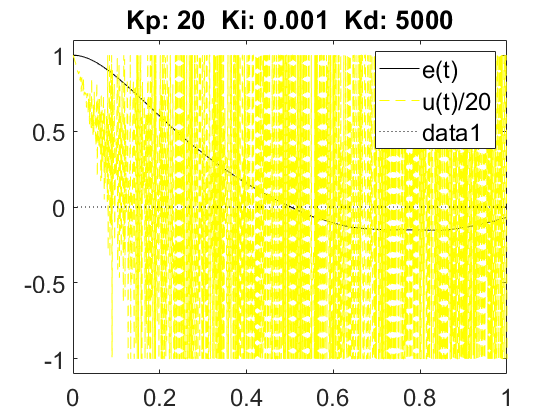
\includegraphics[width=4.8in]{23b.png}

    This result makes sense since the derivative signal that is scaled by $k_d$ is very susceptible to noise, especially before adding a first-order derivative filter and since it is calculated using a simple integration that just considers the last value, thus noise causes massive changes to the derivative effort.

    \item[c.] 

    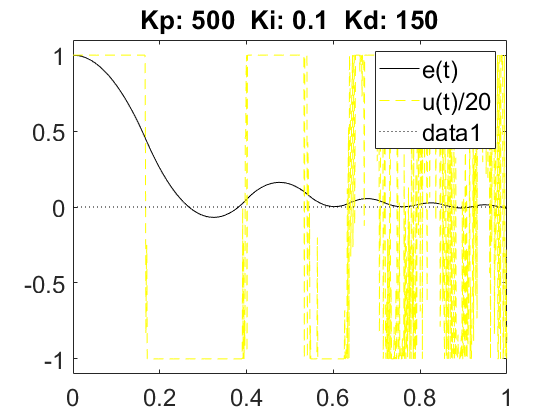
\includegraphics[width=4.8in]{23c.png}

    I was unable to get an exact match to the response in a. since I could not effectively get the damping high enough, but the response is stable and resembles a.. Do note that even though the effort often saturates it doesn't switch as rapidly between effort values like other tested gain values.

    See \verb|pidtest_with_noise_fo_filter.m| for the filtering code added to \verb|pidtest_with_noise.m|.
\end{enumerate}

\end{document}
